\documentclass[aspectratio=169]{beamer}
% \usepackage{pgfpages}
% \pgfpagesuselayout{4 on 1}[a4paper,landscape,border shrink=5mm]
\usepackage{tikz}
\usetikzlibrary{shapes, backgrounds, arrows, positioning}
%\usepackage{pgfplots}
\usepackage{listings}
\usepackage[utf8,latin1]{inputenc}
\usepackage[style = apa, backend = biber, natbib = true]{biblatex}
\addbibresource{../../literature/lit.bib}

\makeatletter \def\newblock{\beamer@newblock} \makeatother  

\beamertemplatenavigationsymbolsempty
\setbeamertemplate{itemize items}[circle]
\setbeamertemplate{section in toc}[circle]
\mode<beamer>{\setbeamercolor{math text displayed}{fg=iwmgray}}
\setbeamercolor{block body}{bg=iwmorange!50!white}
\setbeamercolor{block title}{fg=white, bg=iwmorange}

% Definitions for biblatex
\setbeamercolor{bibliography entry note}{fg=iwmgray}
\setbeamercolor{bibliography entry author}{fg=iwmgray}
\setbeamertemplate{bibliography item}{}


\definecolor{iwmorange}{RGB}{255,105,0}
\definecolor{iwmgray}{RGB}{67,79,79}
\definecolor{iwmblue}{RGB}{60,180,220}
\definecolor{iwmgreen}{RGB}{145,200,110}
\definecolor{iwmpurple}{RGB}{120,0,75}

\setbeamercolor{title}{fg=iwmorange}
\setbeamercolor{frametitle}{fg=iwmorange}
\setbeamercolor{structure}{fg=iwmorange}
\setbeamercolor{normal text}{fg=iwmgray}
\setbeamercolor{author}{fg=iwmgray}
\setbeamercolor{date}{fg=iwmgray}

\title{Random effects for within-subject designs}
\author{Nora Wickelmaier}
\date{Last modified: \today}

\newcommand{\vect}[1]{\mathbf{#1}}
\newcommand{\mat}[1]{\mathbf{#1}}
\newcommand{\gvect}[1]{\boldsymbol{#1}}
\newcommand{\gmat}[1]{\boldsymbol{#1}}

\lstset{language = R,%
  basicstyle = \ttfamily\color{iwmgray},
  frame = single,
  rulecolor = \color{iwmgray},
  commentstyle = \slshape\color{iwmgreen},
  keywordstyle = \bfseries\color{iwmgray},
  identifierstyle = \color{iwmpurple},
  stringstyle = \color{iwmblue},
  numbers = none,%left,numberstyle = \tiny,
  basewidth = {.5em, .4em},
  showstringspaces = false,
  emphstyle = \color{red!50!white}}

\pgfmathdeclarefunction{gauss}{2}{%
  \pgfmathparse{1/(#2*sqrt(2*pi))*exp(-((x-#1)^2)/(2*#2^2))}%
}

\AtBeginSection[]{
  \frame{
    \tableofcontents[sectionstyle=show/hide, subsectionstyle=show/show/hide]}}

\setbeamertemplate{headline}{
 \begin{beamercolorbox}{section in head}
   \vskip5pt\insertsectionnavigationhorizontal{\paperwidth}{}{}\vskip2pt
 \end{beamercolorbox}
}

\setbeamertemplate{footline}{\vskip-2pt\hfill\insertframenumber$\;$\vskip2pt}

\begin{document}

\begin{frame}{}
\thispagestyle{empty}
\titlepage
\end{frame}

% \begin{frame}{Outline}
% \tableofcontents
% \end{frame}

\begin{frame}[<+->]{Selection of random effects}
  \begin{itemize}
    \item How to choose an appropriate random effects structure for a
      mixed-effects model is widely discussed in the literature
      \citep[e.\,g.,][]{Barr2013, Gelman2024, Bates2018}
    \item A prominent view is, that the random effects structure needs to
      represent the experimental design
    \item Leaving out random slopes for the subjects implies that there are no
      individual effects for subjects
    \item Hence, it is assumed that the experimental manipulation has the same
      effect for every subject
  \end{itemize}
\end{frame}

\section{Physical healing}

\begin{frame}[<+->]{Physical healing}{\citep{Aungle2023}}
  \begin{center}
  \begin{tabular}{l|cccc}
    \hline
    Condition & Mean  & SD    & $N_{subjects}$ & $N_{ratings}$ \\
    \hline
    14-min    & 6.17  & 2.59  & 32             &  800 \\
    28-min    & 6.43  & 2.54  & 33             &  825 \\
    56-min    & 7.30  & 2.25  & 32             &  800 \\
    \hline
  \end{tabular}
  \end{center}
  \begin{itemize}
    \item How perceived time influences physical healing
    \item They used cupping to induce bruises on 33 subjects, then took a
      picture, waited for 28\,min and took another picture
    \item Subjects participated in all three conditions over a two week period
    \item Subjective time was manipulated to feel like 14, 28, or 56\,min
    \item Pre and post pictures were presented to 25 raters (amount of healing
      with 0~=~not at all healed, 5~=~somewhat healed, 10~=~completely healed)
  \end{itemize}
\end{frame}

\begin{frame}[<+->]{Possible models}{\citep{Aungle2023}}
  \footnotesize
  \begin{itemize}
    \item Model with random intercepts for subjects and random intercepts for
      raters
  \[
    y_{ij} = \beta_0 + \beta_1 Condition_{28} + \beta_2 Condition_{56} +
      \omega_{0j} + \upsilon_{0i} + \varepsilon_{ij} 
  \]
\small
      with $\upsilon_{0i} \sim N(0, \sigma_{\upsilon}^2)$,
      $\omega_{0j} \sim N(0, \sigma_{\omega}^2)$, $\varepsilon_{ij} \sim N(0,
  \sigma_{\varepsilon}^2)$, all i.i.d. 
    \item Model with random slopes for subjects and random intercepts for
      raters
  \[
    y_{ij} = \beta_0 + \beta_1 Condition_{28} + \beta_2 Condition_{56} +
      \omega_{0j} + \upsilon_{0i} + \upsilon_{1i} Condition_{28} +
      \upsilon_{2i} Condition_{56} + \varepsilon_{ij} 
  \]
\small
with $\gvect{\upsilon} \sim N\left(\gvect{0}, \gmat{\Sigma}_{\upsilon} = 
    \begin{pmatrix}
      \sigma^2_{\upsilon_0} & \sigma_{\upsilon_0\upsilon_1}  & \sigma_{\upsilon_0\upsilon_2}\\
      \sigma_{\upsilon_0\upsilon_1} & \sigma^2_{\upsilon_1}  & \sigma_{\upsilon_1\upsilon_2}\\
      \sigma_{\upsilon_0\upsilon_2} & \sigma_{\upsilon_1\upsilon_2} & \sigma^2_{\upsilon_2} \\
    \end{pmatrix}\right)$,
      $\omega_{0j} \sim N(0, \sigma_{\omega}^2)$, $\varepsilon_{ij} \sim N(0,
  \sigma_{\varepsilon}^2)$, all i.i.d. 
    \item Model with random slope for subjects and random intercepts for
      raters, zero correlations
  \[
    y_{ij} = \beta_0 + \beta_1 Condition_{28} + \beta_2 Condition_{56} +
      \omega_{0j} + \upsilon_{0i} + \upsilon_{1i} Condition_{28} +
      \upsilon_{2i} Condition_{56} + \varepsilon_{ij} 
  \]
\small
with $\gvect{\upsilon} \sim N\left(\gvect{0}, \gmat{\Sigma}_{\upsilon} = 
    \begin{pmatrix}
      \sigma^2_{\upsilon_0} & 0  & 0\\
      0 & \sigma^2_{\upsilon_1}  & 0\\
      0 & 0 & \sigma^2_{\upsilon_2} \\
    \end{pmatrix}\right)$,
      $\omega_{0j} \sim N(0, \sigma_{\omega}^2)$, $\varepsilon_{ij} \sim N(0,
  \sigma_{\varepsilon}^2)$, all i.i.d. 
  \end{itemize}
\end{frame}

\begin{frame}[fragile]{Model comparisons}{\citep{Aungle2023}}
  \begin{columns}
    \begin{column}{.69\textwidth}
\begin{lstlisting}
library("lme4")
load("data/healing.RData")

m1 <- lmer(Healing ~ Condition +
  (1 | Subject) + (1 | ResponseId), dat)
m2 <- lmer(Healing ~ Condition +
  (Condition | Subject) + (1 | ResponseId), dat)
m3 <- lmer(Healing ~ Condition +
  (dummy(Condition, "28") +
   dummy(Condition, "56") || Subject) +
  (1 | ResponseId), dat)
\end{lstlisting}
    \end{column}
    \begin{column}{.35\textwidth}
      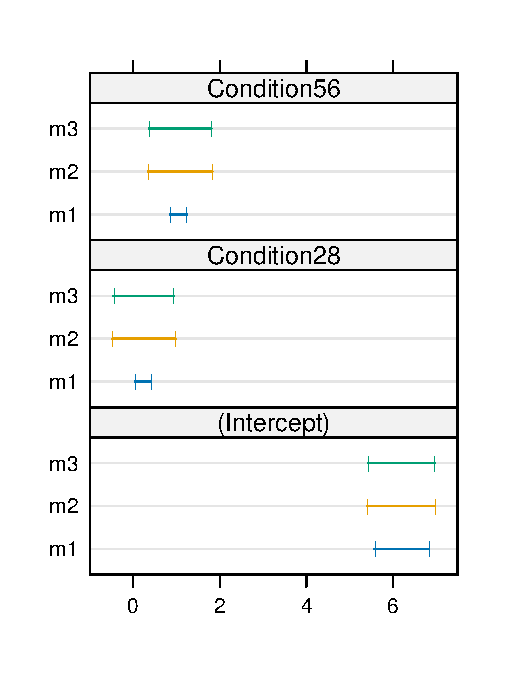
\includegraphics[scale=.6]{../figures/heal_ci}
    \end{column}
  \end{columns}
\end{frame}

\begin{frame}[fragile]{Different random effects}
  {Random intercept model}
  \begin{itemize}
    \item What is the difference between these 3 models?
  \end{itemize}
\begin{lstlisting}
lapply(coef(m1), head, n = 3)
# $Subject
#        (Intercept) Condition28 Condition56
# 111191    5.759678   0.2272593    1.047163
# 117694    7.245319   0.2272593    1.047163
# 141451    4.276601   0.2272593    1.047163
# 
# $ResponseId
#                   (Intercept) Condition28 Condition56
# R_1DZrj0mXFNlzerG    3.160095   0.2272593    1.047163
# R_1F99W1Qnk3uLGTg    5.440917   0.2272593    1.047163
# R_1I4p00HhjngCBwT    3.914327   0.2272593    1.047163
\end{lstlisting}
\end{frame}

\begin{frame}[fragile]{Different random effects}
  {Random slope model}
  \begin{itemize}
    \item What is the difference between these 3 models?
  \end{itemize}
\begin{lstlisting}
lapply(coef(m2), head, n = 3)
# $Subject
#        (Intercept) Condition28 Condition56
# 111191    4.517425   0.9372819   4.0356794
# 117694    7.480483  -0.1545164   0.7669798
# 141451    3.717059   1.2029451   1.6695395
# 
# $ResponseId
#                   (Intercept) Condition28 Condition56
# R_1DZrj0mXFNlzerG    3.115764   0.2462495    1.089368
# R_1F99W1Qnk3uLGTg    5.415579   0.2462495    1.089368
# R_1I4p00HhjngCBwT    3.876277   0.2462495    1.089368
\end{lstlisting}
\end{frame}

\begin{frame}[fragile]{Different random effects}
  {Random slope model without correlations}
  \begin{itemize}
    \item What is the difference between these 3 models?
  \end{itemize}
\begin{lstlisting}
lapply(coef(m3), head, n = 3)
# $Subject
#        dummyCond28 dummyCond56 (Intercept) Condition28 Condition56
# 111191   0.5508955   2.8897054    4.596686   0.2390194    1.083531
# 117694  -0.3384845  -0.2573444    7.455698   0.2390194    1.083531
# 141451   0.8596727   0.4654271    3.768399   0.2390194    1.083531
# 
# $ResponseId
#                   (Intercept) Condition28 Condition56
# R_1DZrj0mXFNlzerG    3.123060   0.2390194    1.083531
# R_1F99W1Qnk3uLGTg    5.422826   0.2390194    1.083531
# R_1I4p00HhjngCBwT    3.883556   0.2390194    1.083531
\end{lstlisting}
\end{frame}

\begin{frame}[<+->]{Summary}
  \begin{itemize}
    \item When we use mixed-effects models to fit data, we need to make an
      informed choice about the random effects we include in the model
    \item Complex random effect structures can lead to convergence problems and
      variance terms for random slopes are not always easy to estimate
    \item The random effects structure strongly influences the confidence
      intervals for the fixed effects which we are often interested in
    \item This is especially relevant in a confirmatory setting
    \item For some critical discussion of the healing paper and their choice of
      random effects see \citet{Gelman2024} and Gelman's blog post and
      discussion here:
      \url{https://statmodeling.stat.columbia.edu/2025/01/23/slopes/}
  \end{itemize}
\end{frame}

\section[AIES]{Perceived risk of AI expert systems}

\begin{frame}[fragile]{Perceived risk of AI expert systems}
  Independent variables
  \begin{itemize}
    \item Participant ($N = 898$)
    \item Partner (AI vs.\ hu, within)
    \item Stakes (HS vs.\ LS, within)
    \item Context (edu vs.\ fin vs.\ law vs.\ med vs.\ psy, between)
  \end{itemize}
  Dependent variables
  \begin{itemize}
    \item Perceived risk (1 item, 7-point scale, from ``None at all'' to
      ``Maximally'')
    \item Perceived trustworthiness (9 items, 7-point scale, averaged)
  \end{itemize}
  \begin{lstlisting}
dat <- read.table("data/data-nico.csv", sep = ",", header = TRUE,
                  stringsAsFactors = TRUE)
  \end{lstlisting}
\end{frame}

\begin{frame}[<+->]{Choose a mixed-effects model}
  \begin{itemize}
    \item Let us look at perceived risk
    \item Hypothesis: In certain contexts, people will perceive the risk to
      consult an AI expert sytem as much higher compared to a human expert when
      stakes are high
      % we hypothesize that stakes (low vs. high) involved significantly
      % influences perceived risk in certain contexts (H2)
    \item Draw a hypothesis plot
    \item What mixed-effects model is suited to test this hypothesis?
    \item How many parameters does this model have?
    \item Which parameter do we need to look at in order to test the hypothesis?
    \item Which random effects are needed to represent the experimental design?
  \end{itemize}
\end{frame}

\begin{frame}[fragile]{Testing three-way interaction}
  \begin{lstlisting}
m0 <- lmer(Risk ~ (Context + Partner + Stakes)^2 +
           (1 + Partner + Stakes | Participant), data = dat)

m1 <- lmer(Risk ~ Context * Partner * Stakes +
           (1 + Partner + Stakes | Participant), data = dat)

# Test interaction with Likelihood-ratio Test
anova(m0, m1)
  \end{lstlisting}
  \pause
  \begin{itemize}
    \item Calculate the confidence intervals for Model \texttt{m1} and compare
      them to a model with only random intercepts for \texttt{Participant}
    \item What would you expect based on the results we looked at for
      \citet{Aungle2023}?
  \end{itemize}
\end{frame}

\begin{frame}{Confidence intervals for three way interaction}
  \begin{center}
    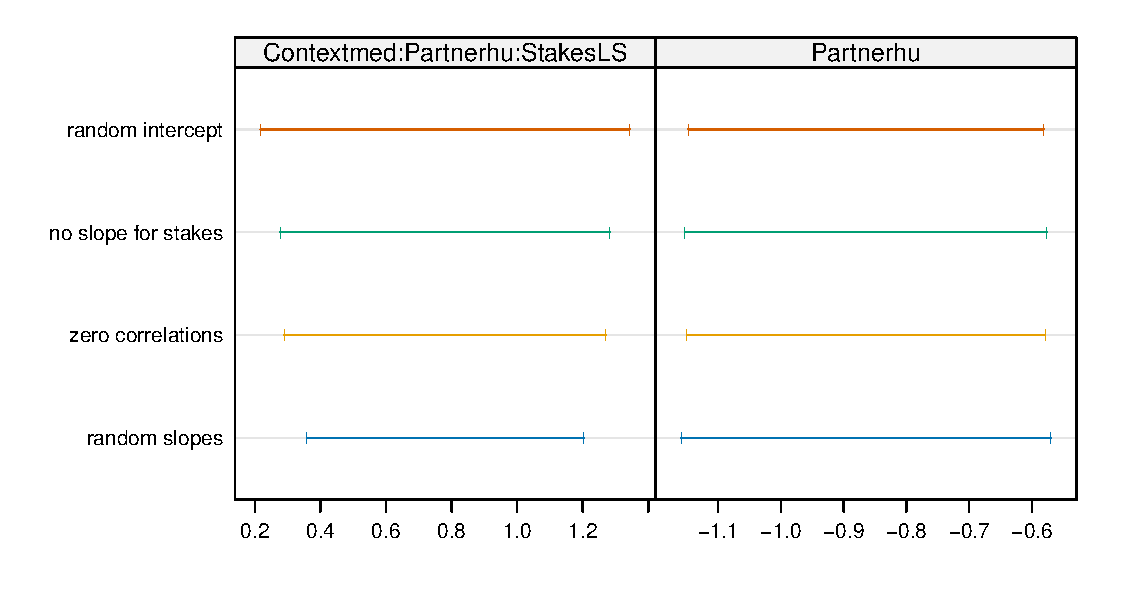
\includegraphics[scale=.7]{../figures/nico_cis_data-risk}
  \end{center}
\end{frame}

\section{Simulations}

\begin{frame}[<+->]{Selection of random effects}
  \begin{itemize}
    \item What is the difference between the two designs we looked at?
    \item Maybe it's just one of the data sets behaving weird?
    \item Let's check and simulate some data \dots
  \end{itemize}
\end{frame}

\begin{frame}[fragile]{$2\times 2$ within design}
  \[
    y = \beta_0 + \beta_1 a_2 + \beta_2 b_2 + \beta_3 a_2b_2 +
        \upsilon_0 + \upsilon_1 a_2 + \upsilon_2 b_2 + \varepsilon
  \]
  with $\gvect{\upsilon} \sim N\left(\gvect{0}, \gmat{\Sigma}_{\upsilon} = 
    \begin{pmatrix}
      \sigma^2_{\upsilon_0} & \sigma_{\upsilon_0\upsilon_1}  & \sigma_{\upsilon_0\upsilon_2}\\
      \sigma_{\upsilon_0\upsilon_1} & \sigma^2_{\upsilon_1}  & \sigma_{\upsilon_1\upsilon_2}\\
      \sigma_{\upsilon_0\upsilon_2} & \sigma_{\upsilon_1\upsilon_2} & \sigma^2_{\upsilon_2} \\
    \end{pmatrix}\right)$, $\varepsilon_{ij} \sim N(0, \sigma_{\varepsilon}^2)$,
    all i.i.d.
    \vspace{.5cm}
  \small
  \begin{lstlisting}
dat <- expand.grid(A = factor(c("a1", "a2")), B = factor(c("b1", "b2")),
                   id = factor(1:10))

beta  <- c(3, .5, .5, 1)
sp    <- c(1, .8, .6)
r     <- -.5
S     <- r * sp %o% sp; diag(S) <- sp^2
se    <- 1
  \end{lstlisting}
\end{frame}


\begin{frame}[fragile]{$2\times 2$ within design}
  \footnotesize
  \begin{lstlisting}
Lt    <- chol(S) / se
theta <- t(Lt)[lower.tri(Lt, diag = TRUE)]

cis <- replicate(100, {
  y <- simulate(~ A * B + (A + B | id),
                newdata = dat,
                newparams = list(beta = beta, theta = theta, sigma = se))$sim_1
  m0 <- lmer(y ~ A * B + (1 | id), dat)
  m1 <- lmer(y ~ A * B + (A + B | id), dat)
  matrix(c(confint(m0, par = "Aa2:Bb2", method = "Wald") |> as.numeric(),
           confint(m1, par = "Aa2:Bb2", method = "Wald") |> as.numeric()),
         nrow = 2, byrow = TRUE)
  }, simplify = FALSE
)
dat_ci <- as.data.frame(do.call(rbind, cis))
names(dat_ci) <- c("lb", "ub")
dat_ci$model <- factor(c("random intercept", "random slope"))
  \end{lstlisting}
\end{frame}

\begin{frame}{$2\times 2$ within design}
  \begin{columns}
    \begin{column}{.5\textwidth}
      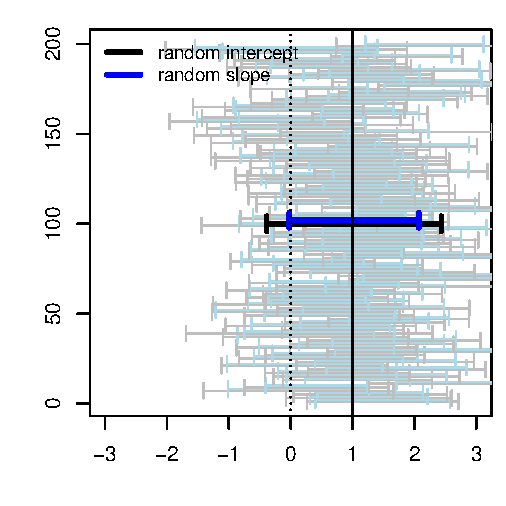
\includegraphics[scale=.8]{../figures/nico_cis_2x2design_1obs}
    \end{column}
    \begin{column}{.5\textwidth}
      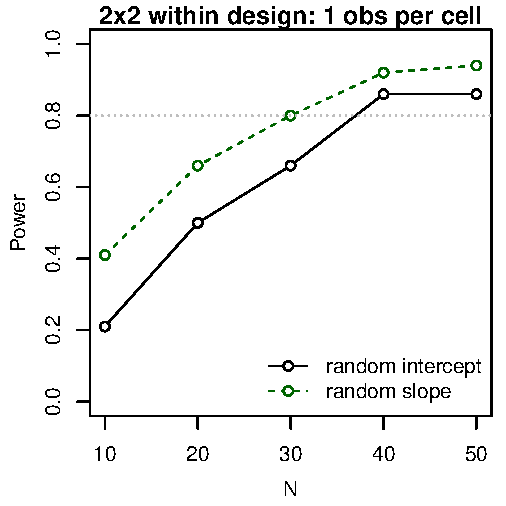
\includegraphics[scale=.8]{../figures/nico_power_2x2design_1obs}
    \end{column}
  \end{columns}
\end{frame}

\begin{frame}[fragile]{$2\times 2$ within design with several items}
  \small
  \[
    y = \beta_0 + \beta_1 a_2 + \beta_2 b_2 + \beta_3 a_2b_2 +
        \upsilon_0 + \upsilon_1 a_2 + \upsilon_2 b_2 + \upsilon_3 a_2b_2 +
        \omega_0 + \varepsilon
  \]
  with $\gvect{\upsilon} \sim N\left(\gvect{0}, \gmat{\Sigma}_{\upsilon} = 
    \begin{pmatrix}
      \sigma^2_{\upsilon_0} & \sigma_{\upsilon_0\upsilon_1}  & \sigma_{\upsilon_0\upsilon_2} & \sigma_{\upsilon_0\upsilon_3}\\
      \sigma_{\upsilon_0\upsilon_1} & \sigma^2_{\upsilon_1}  & \sigma_{\upsilon_1\upsilon_2} & \sigma_{\upsilon_1\upsilon_3}\\
      \sigma_{\upsilon_0\upsilon_2} & \sigma_{\upsilon_1\upsilon_2} & \sigma^2_{\upsilon_2}  & \sigma_{\upsilon_2\upsilon_3}\\
      \sigma_{\upsilon_0\upsilon_3} & \sigma_{\upsilon_1\upsilon_3} & \sigma_{\upsilon_2\upsilon_3}  & \sigma^2_{\upsilon_3}\\
    \end{pmatrix}\right)$,
    $\omega_{0} \sim N(0, \sigma_{\omega}^2)$,
    $\varepsilon_{ij} \sim N(0, \sigma_{\varepsilon}^2)$
    \vspace{.5cm}
    \begin{lstlisting}
dat <- expand.grid(A = factor(c("a1", "a2")), B = factor(c("b1", "b2")),
                   item = factor(1:5), id = factor(1:10))
beta   <- c(3, .5, .5, 1)
sp     <- c(1, .8, .6)
r      <- -.5
se     <- 1
S      <- r * sp %o% sp; diag(S) <- sp^2
sw     <- 1
    \end{lstlisting}
\end{frame}

\begin{frame}{$2\times 2$ within design with several items}
  \begin{columns}
    \begin{column}{.5\textwidth}
      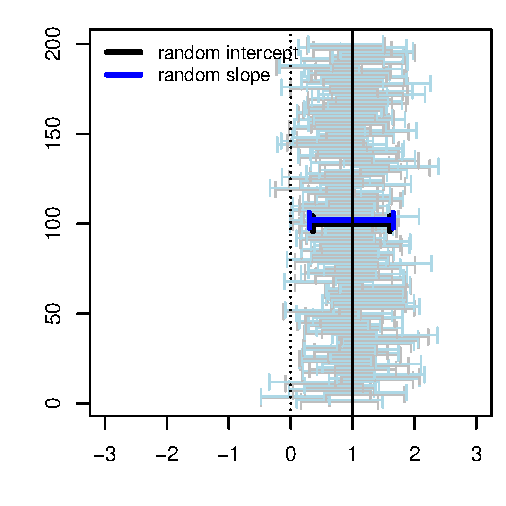
\includegraphics[scale=.8]{../figures/nico_cis_2x2design_5obs}
    \end{column}
    \begin{column}{.5\textwidth}
      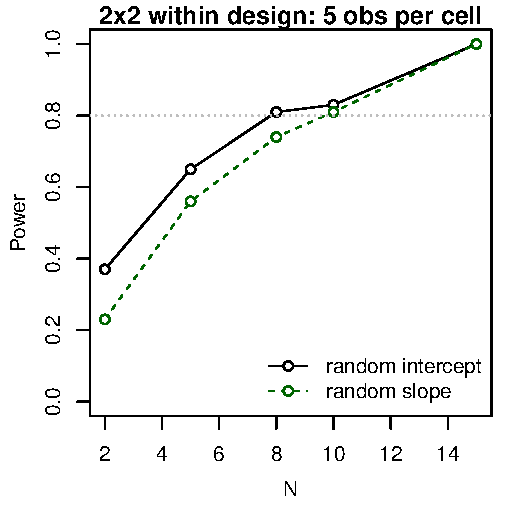
\includegraphics[scale=.8]{../figures/nico_power_2x2design_5obs}
    \end{column}
  \end{columns}
\end{frame}

\begin{frame}[<+->]{Summary}
  \begin{itemize}
    \item The discussion ``Keep it maximal'' \citep{Barr2013} vs.\
      ``Parsimonious mixed models'' \citep{Bates2018} is even more complicated
      than it looks (as always)
    \item I still think that the random effects structure should represent the
      experimental design, since this aligns with thinking about the structure
      of the random effects as the data generating process
    \item If you want to interpret the random effects or even test hypotheses
      about them, you need to be careful if the estimates are good enough,
      however
    \item And always: Do not go through the motions, try to understand the
      model that you fit and what its structure implies
  \end{itemize}
\end{frame}

\appendix

%\begin{frame}[allowframebreaks]{References}
\begin{frame}{References}
  %\renewcommand{\bibfont}{\footnotesize}
  \printbibliography
  %\vfill
\end{frame}

\end{document}

